\documentclass{proc}
\usepackage{url}
\usepackage{graphicx}
\usepackage{todonotes}
\usepackage{mathtools}

\begin{document}

\title{Perception and Language:  popular discourses in uncertainty and probability visualizations}

%\title{color-based perception of risk}
%We vary the color, maps projection, scale, and see how people classify the situation as risky...

\author{Author1, Author2}

\maketitle

%----------------------------------------------------------SECTION---------
\section{Introduction}
 %\cite{dragicevic2016fair}
We encounter different forms of visualizations in many aspects of our daily lives and there are different factors that influence how we interact with or make use of them. For e.g., information about the designers or the data origin can influence the trust that viewers have in a particular visualization \cite{peck2019data}, social information such as popular trends or choices can influence our visual judgments\cite{hullman2011impact}, literacy, familiarity with charts or with the interface design \cite{blascheck2018exploration} can influence the way we interact with a visualization system, search for and extract information from it, the diversity of languages and terminologies for visual components such as colors \cite{lindsey2009world} could explain how visualizations are built across cultures and countries. 

Visualization can be a powerful tool for empowering people and supporting them in their decision-making. However, the knowledge and information contained in data and encoded in the visuals need to be communicated in order to make them actionable. Language is an important tool used to formulate and communicate the content of a visualization. When working with complex visualizations such as those that embed uncertainty, or show critical information, the different terminologies used among groups, across cultures and geographical location, can make the same message ambiguous. 

In this experiment, we make the following contributions: 
\begin{itemize}
    \item we study the discourse that people structure and use to communicate the information they perceive in uncertainty or probability in visualizations. 
    \item \textbf{possible possible contribution} compare the discourses across languages. 
\end{itemize}
 
% \url{https://www.visualcapitalist.com/measuring-perceptions-of-uncertainty/}

\section{One-sentence description}
Study of the language that people use to describe probability, uncertainty in visualizations.
%Analyzing people's behaviors towards specific visualizations help us understand how language and discourse shape the understanding or communication of findings in visualization -- how people understand concepts in vis and which discourse they use to communicate them. 

%----------------------------------------------------------SECTION---------
\section{Project Type}
Crowdsourcing, Online large experiment.

%----------------------------------------------------------SECTION---------
\section{Audience} 
\begin{quote}
\textit{Who is the audience for this project? 
How does it meet their needs? 
What happens if their needs remain unmet?}
\end{quote}
The audience of the project is anyone who encounters data visualizations in their daily lives, uses them to make decisions, but especially to explain or communicate findings. It is necessary to know the popular discourse used to communicate or describe critical visualization. Understanding the language one uses or others use for describing graphs and phenomena such as uncertainty, risk or probability can help people make informed personal or collective decisions. %(putting words on graphs or graphs on words)

%----------------------------------------------------------SECTION---------
\section{Approach}
The experiment will be conducted using online crowdsourcing, during which participants will be shown a graph at a time as well as a collection of words that describe probability or likelihood. Participant will then choose the word they think best matches the visualization or select the part of the visualization that they think best corresponds to a given word. 

\subsection{Graphs}
We will use three types of graphs: 

\begin{itemize}
    \item \textbf{simple graphs}: (or basic shapes) barcharts, pie charts as in in Cleveland et al.'s experiment \cite{cleveland1984graphical}
    \item \textbf{more complex plots}: box plots, sinaplots\cite{sidiropoulos2018sinaplot}?
    \item \textbf{usual visualizations}: these are graphs that show uncertainty (e.g. weather forecasts) or other types that people encounter more in daily lives and that use forecasting languages.  
\end{itemize}

\subsection{Words}
We will use the 17 probability words in Sherman's study of the perception of uncertainty \cite{desjardins2017measuring}.


Figure \ref{exp-interface1} shows an example of interface for the experiment in which the user is presented a choice of probability words to choose among.  
Other forms of questions are shown in Figures \ref{exp-interface2} and \ref{weather-unc2} where the user selects the visualization they think best fit to a probability word. 

\begin{figure}[!t]
    \centering
    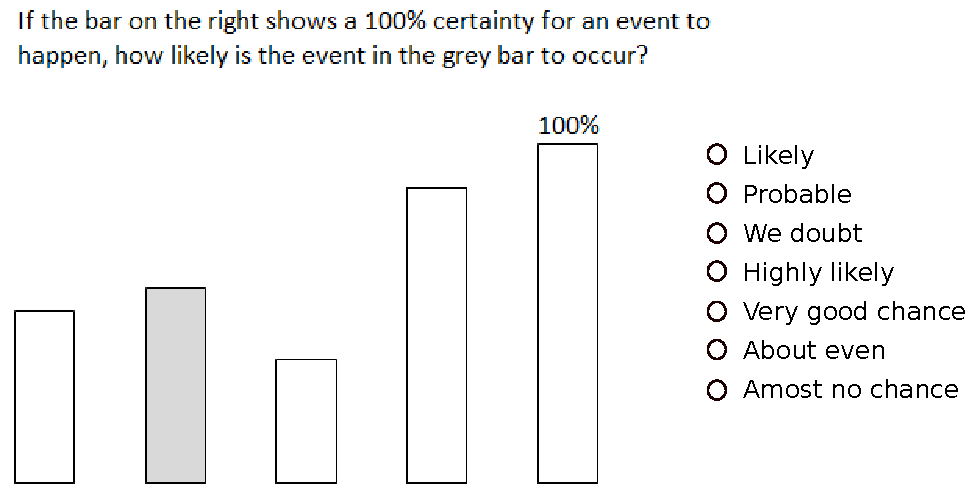
\includegraphics[width=\columnwidth]{figures/exp-int1.pdf}
    \caption{Experiment interface example 1}
    \label{exp-interface1}
\end{figure}

\begin{figure}[!t]
    \centering
    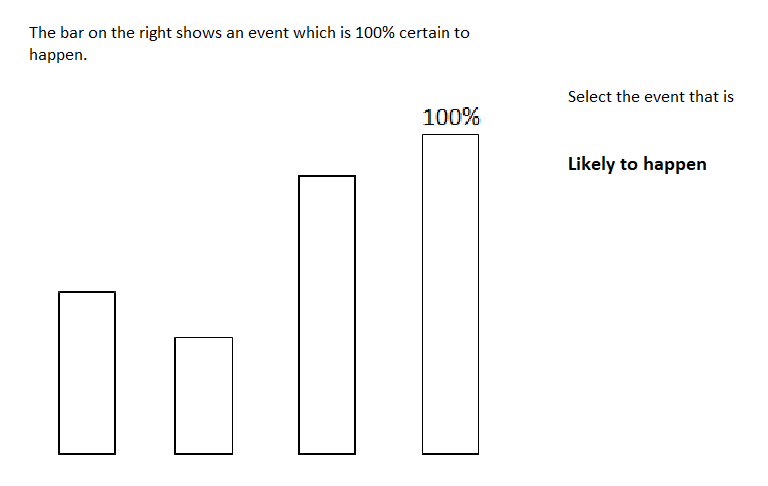
\includegraphics[width=\columnwidth]{figures/exp-int2.png}
    \caption{Experiment interface example 2}
    \label{exp-interface2}
\end{figure}

\begin{figure}[!t]
    \centering
    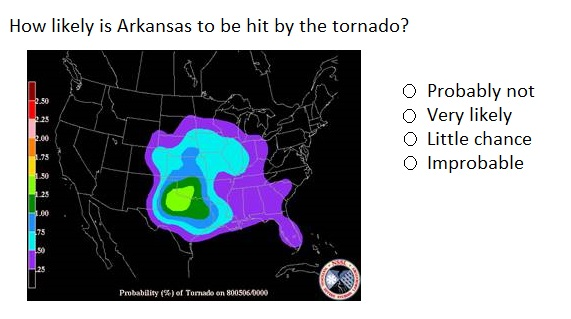
\includegraphics[width=\columnwidth]{figures/weather-uncertainty2.jpg}
    \caption{Experiment interface example 3, source: http://www.spc.noaa.gov/products/}
    \label{weather-unc2}
\end{figure}

%---------------------------------------------------------subsection-------
\subsection{Details}
\begin{quote}
\textit{What is your approach?}
\end{quote}

Trial + real experiments. Trial objectives: train subjects on how to read visualization.

\todo[inline]{find paper on Sherman's work if any?}
We use the analysis by Sherman \cite{desjardins2017measuring} and the one in \cite{zonination} as a baseline to compare the data which we'll collect. These studies already provides an association of numbers and expressions as shown in Figure \ref{perceptions-of-probability}.

\begin{figure}[!t]
    \centering
    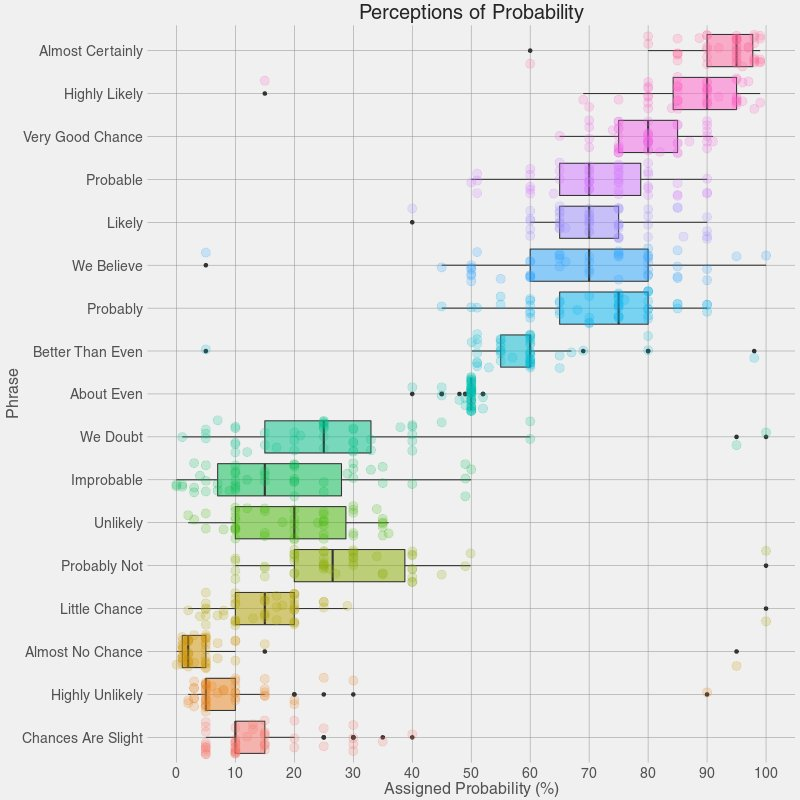
\includegraphics[width=\columnwidth]{figures/perceptions-of-probability.jpg}
    \caption{Perceptions of probability, source: \cite{zonination}}
    \label{perceptions-of-probability}
\end{figure}
\todo[inline]{Research paper on Zonination's study?}

We will visualize the range of probability numbers in these studies and ask questions that help us identify whether the same languages are used when the probabilities are shown in graphs not in numbers. 

\todo[inline]{Cross-language study if time permits $\downarrow$}
We will select one or more reference dictionaries for translating the different probability expressions (e.g. \url{https://dictionary.cambridge.org/}) and run a translated version of the experiment. A (ideal?) possibility could be that a bilingual participant conducts the experiment in two different languages. Such data would inform us on how the different expressions are used in different languages by a same individual. 

%---------------------------------------------------------subsection-------
\subsection{Evidence for Success}
\begin{quote}
\textit{Why do you think it will work?} 

\end{quote}

%----------------------------------------------------------SECTION---------
\section{Best-case Impact Statement}
\begin{quote}
\textit{In the best-case scenario, what would be the impact statement (conclusion statement) for this project?}
\end{quote}
Ideally: "We found that people use to describe the probability and uncertainty in visualizations are (not) the same as what they use in perceptions of numbers." OR (for e.g.) "While in previous studies, the term X was associated to probability range [p1, p2], when represented in graphs, the same term is used by people to describe probabilities in range [p'1, p'2]."

\todo[inline]{cross-language conclusion if time permits $\downarrow$}
By observing the data, we conclude that the probability word "X" (associated to probability range [x1, x2]) has it translation in \textit{other-language-name-here} "XX" .

\section{Major Milestones}

%Beside selecting  the crowdsourcing platform to use and learning more about crowdsourcing techniques or design, mostly via readings and literature search: 
\begin{itemize}
    \item setup the platforms to use: crowdsourcing (AMT, Prolific), database, app hosting (heroku, glitch?) 
    \item decide which type of charts to use (barcharts \& piehcarts only? boxplots, sinaplots, wheather visualizations or infographics? ) then collect or make them.
    
    \item prepare questions and scenarios (e.g. estimation of probability or  forecasting with uncertainty)
	\item deploy experiment(run tests, run main experiments)
	\item data analysis and draw conclusion
\end{itemize}

%----------------------------------------------------------SECTION---------
\section{Obstacles}

\subsection{Major obstacles} % (if these fail, the project is over)
\begin{itemize}
    \item not sufficient participants to draw conclusion from
    \item 
\end{itemize}
\subsection{Minor obstacles}
\begin{itemize}
    \item getting the actual data from sherman's study instead of merely extrapolating from the published graph.
\end{itemize}
%----------------------------------------------------------SECTION---------
\section{Resources Needed}
\begin{quote}
\textit{What additional resources do you need to complete this project?}
\end{quote}
\begin{itemize}
    \item Prolific account?
\end{itemize}

%----------------------------------------------------------SECTION---------
\section{Related Work}
\begin{quote}
\textit{List 5 major publications that are most relevant to this project, and how they are related (sample citation).}
\end{quote}

Papers that studied external influences on our visual perceptions and on how we build or trust visualizations $\rightarrow$
Hullman et al.'s work~\cite{hullman2011impact} shows how external factors such as social information influence our visual perceptions. They show how people responses to visual stimuli are biased by the knowledge of how other have judged or reacted to the same charts. 

Papers that studied cultural influences on our behaviors towards data visualization $\rightarrow$ 
The work of Lindsay et al.'s work~\cite{lindsey2009world} show how visualization aspects such as the naming of colors may vary across different languages. 

Peck et al.'s work~\cite{peck2019data} analysed how individuals react to or question their trust in charts based on their personal experience or personal connection to the context of the data. In their experiment, some participants asked to review their analysis of a chart once the sources of the data were revealed.

Harrison et al.'s work~\cite{harrison2012exploring} showed how people's judgments and performances during visualization tasks vary based on the type (positive vs negative) priming stories that they are given before executing the tasks. 

The works above address examples of the different factors external to the visualization user that can influence their perception. Internal factors such as language, habits and culture also play important role in how we interpret concepts such as uncertainty. 

Sherman Kent has studied the perception of uncertainty among NATO officers \cite{desjardins2017measuring}. His results has shown the different quantitative value of likelihood that the sample assign to 17 probability words. His study has been generalized in another study which has shown similar results \footnote{\url{https://github.com/zonination/perceptions}} for samples that are more general population. 

These studies show the words that we associate to probabilities in numbers.
However, when it comes to visualization of such uncertainty and probability, people generally do not use exact numbers to describe the information they perceive. In our study we explore the different wording, expression or language that people associate to visualizations that encode uncertainty or probabilities. 


%----------------------------------------------------------SECTION---------
\section{Define Success}
\begin{quote}
\textit{What is the minimum amount of work necessary for this work be publishable?}
\end{quote}
For this work to be publishable, we need: 
\begin{itemize}
    \item enough data to draw conclusion from, at least as many participants as in Sherman's study (23 individuals)
\end{itemize}

\bibliographystyle{abbrv}
\bibliography{prospectus}
\end{document}
